\part{动态规划}

\chapter{动态规划}

\section{线性动规}
\entrymeta{$O(n\log n)$（LIS）}
\subsection{最长上升子序列}\label{ux6700ux957fux4e0aux5347ux5b50ux5e8fux5217}






\begin{codeline}
#define N 1000005
int n;
int num[N];
int d[N];
int main() {
    ios::sync_with_stdio(false);
    cin.tie(nullptr);
    cin >> n;
    int l = 0;
    for(int i = 0; i < n; i++) {
        cin >> num[i];
    }

    l = 1;
    d[0] = num[0];
    int idx;
    int ans = 1;
    for(int i = 1; i < n; i++) {
        if(num[i] > d[l - 1]) {
            d[l] = num[i];
            l++;
        } else {
            idx = lower_bound(d, d + l, num[i]) - d;
            d[idx] = num[i];
        }
        ans = max(ans, l);
    }
    cout << (ans) << '\n';
}
\end{codeline}


\subsection{P1439 两个排列的最长公共子序列}\label{p1439-ux4e24ux4e2aux6392ux5217ux7684ux6700ux957fux516cux5171ux5b50ux5e8fux5217}






\begin{codeline}
const int N = 100005;
int inv[N];
int a[N];
int dp[N];
int main() {
    ios::sync_with_stdio(false);
    cin.tie(nullptr);
    int n, num;
    cin >> n;
    for(int i = 1; i <= n; i++) {
        cin >> num;
        inv[num] = i;
        dp[i] = 0x3f3f3f3f;
    }

    for(int i = 1; i <= n; i++) {
        cin >> num;
        num = inv[num];
        a[i] = num;
    }

    for(int i = 1; i <= n; i++) {
        int j = lower_bound(dp, dp + i, a[i]) - dp;
        j--;
        if(dp[j] < a[i] && a[i] < dp[j + 1]) {
            dp[j + 1] = a[i];
        }
    }

    int ans = 0;
    for(int i = n; i > 0; i--) {
        if(dp[i] != 0x3f3f3f3f) {
            ans = i;
            break;
        }
    }

    cout << (ans);
}
\end{codeline}


\subsection{图片题例：概率 DP}\label{ux56feux7247ux9898ux4f8bux6982ux7387-dp}

此题输入格式见原图，无独立文本样例。

\begin{center}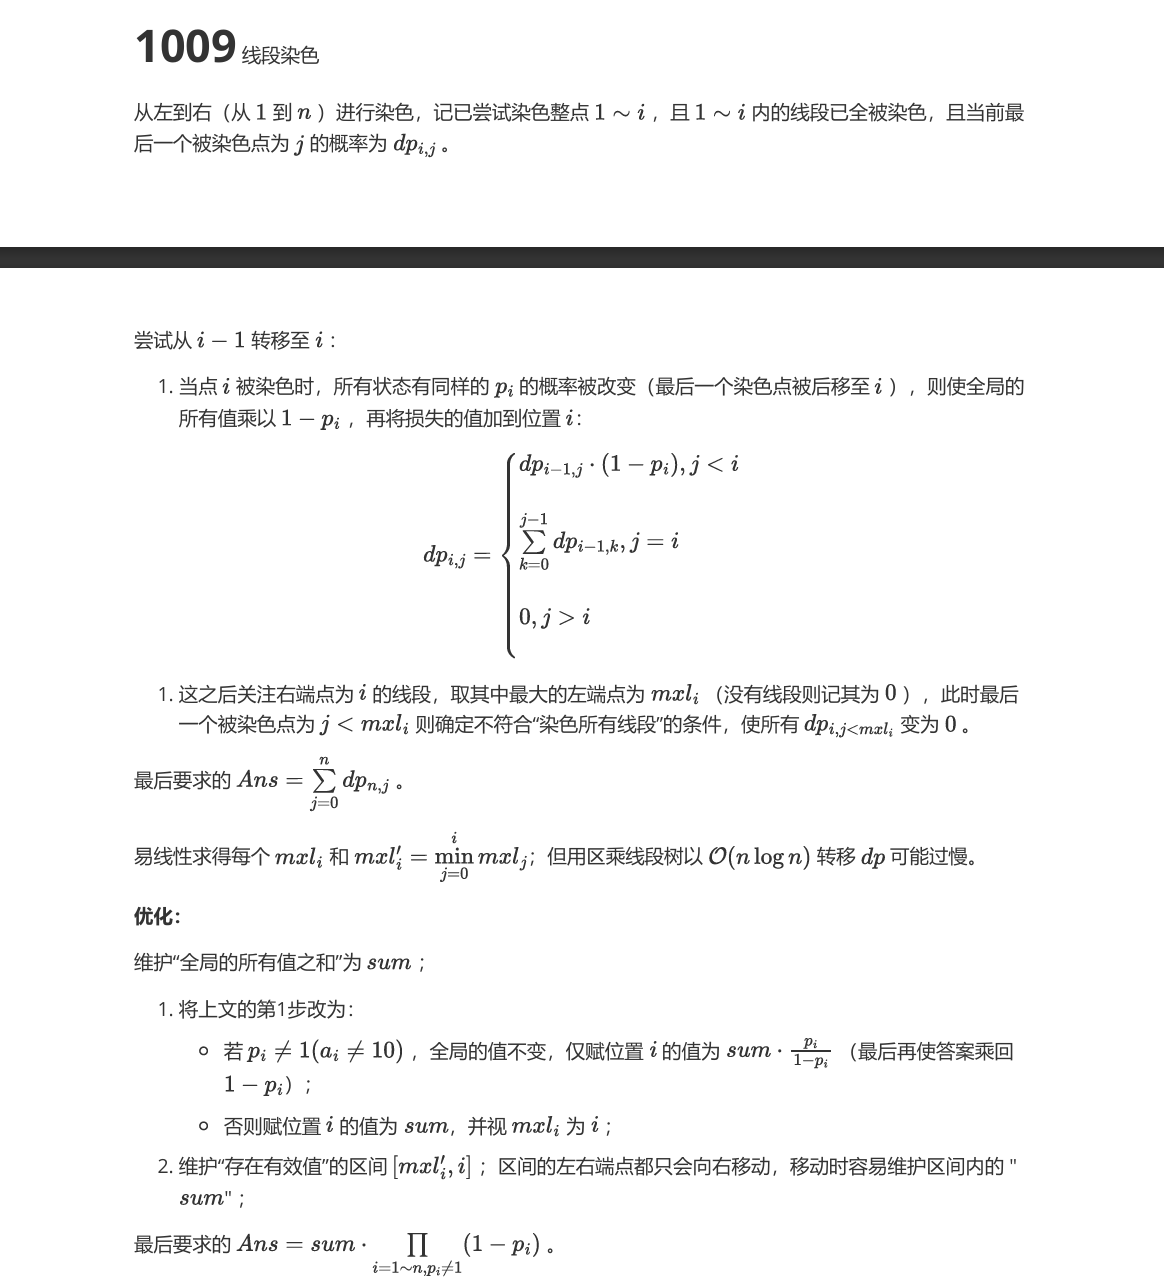
\includegraphics[width=0.78\linewidth]{assets/e061_image-1.png}\end{center}

依赖：\href{../公共/扩展欧几里得.md}{扩展欧几里得·代码块 1}。


\begin{codeline}
const int MODER = 1000000007;
const int N = 200005;
const int INF = 0x3f3f3f3f;

long long inv[11];
long long dp[N];
int p[N];
int maxl[N];

int n, m;

int main() {
    ios::sync_with_stdio(false);
    cin.tie(nullptr);
    for(int i = 1; i <= 10; i++) {
        int64 y;
        exgcd(i, MODER, inv[i], y);
        inv[i] = (inv[i] % MODER + MODER) % MODER;
    }

    int T;
    cin >> T;
    while(T--) {
        cin >> n;
        cin >> m;
        long long pie = 1;
        for(int i = 1; i <= n; i++) {
            cin >> p[i];
            maxl[i] = 0;
            dp[i] = 0;
            if(p[i] != 10) {
                pie = pie * (10 - p[i]) % MODER * inv[10] % MODER;
            }
        }

        dp[0] = 1;

        int l, r;
        for(int i = 0; i < m; i++) {
            cin >> l;
            cin >> r;
            maxl[r] = max(maxl[r], l);
        }

        long long sum = 1;
        l = 0;
\end{codeline}
\vspace{-0.9\baselineskip}
\begin{codeline}[firstnumber=47]

        for(int i = 1; i <= n; i++) {
            if(p[i] != 10) {
                dp[i] = sum * p[i] % MODER * inv[10 - p[i]] % MODER;
                sum = (sum + dp[i]) % MODER;

                if(maxl[i] > l) {
                    for(; l < maxl[i]; l++) {
                        sum -= dp[l];
                        dp[l] = 0;
                    }
                    sum = (sum % MODER + MODER) % MODER;
                }
            } else {
                dp[i] = sum;
                for(; l < i; l++) {
                    dp[l] = 0;
                }
            }
        }
        sum = sum * pie % MODER;

        cout << (sum) << '\n';
    }
}
\end{codeline}
\begin{warnbox}
LIS 用 \texttt{lower\_bound} 求严格上升；\texttt{n = 0} 需单独处理。
\end{warnbox}
\clearpage
\subsection*{延伸阅读}
\begin{center}
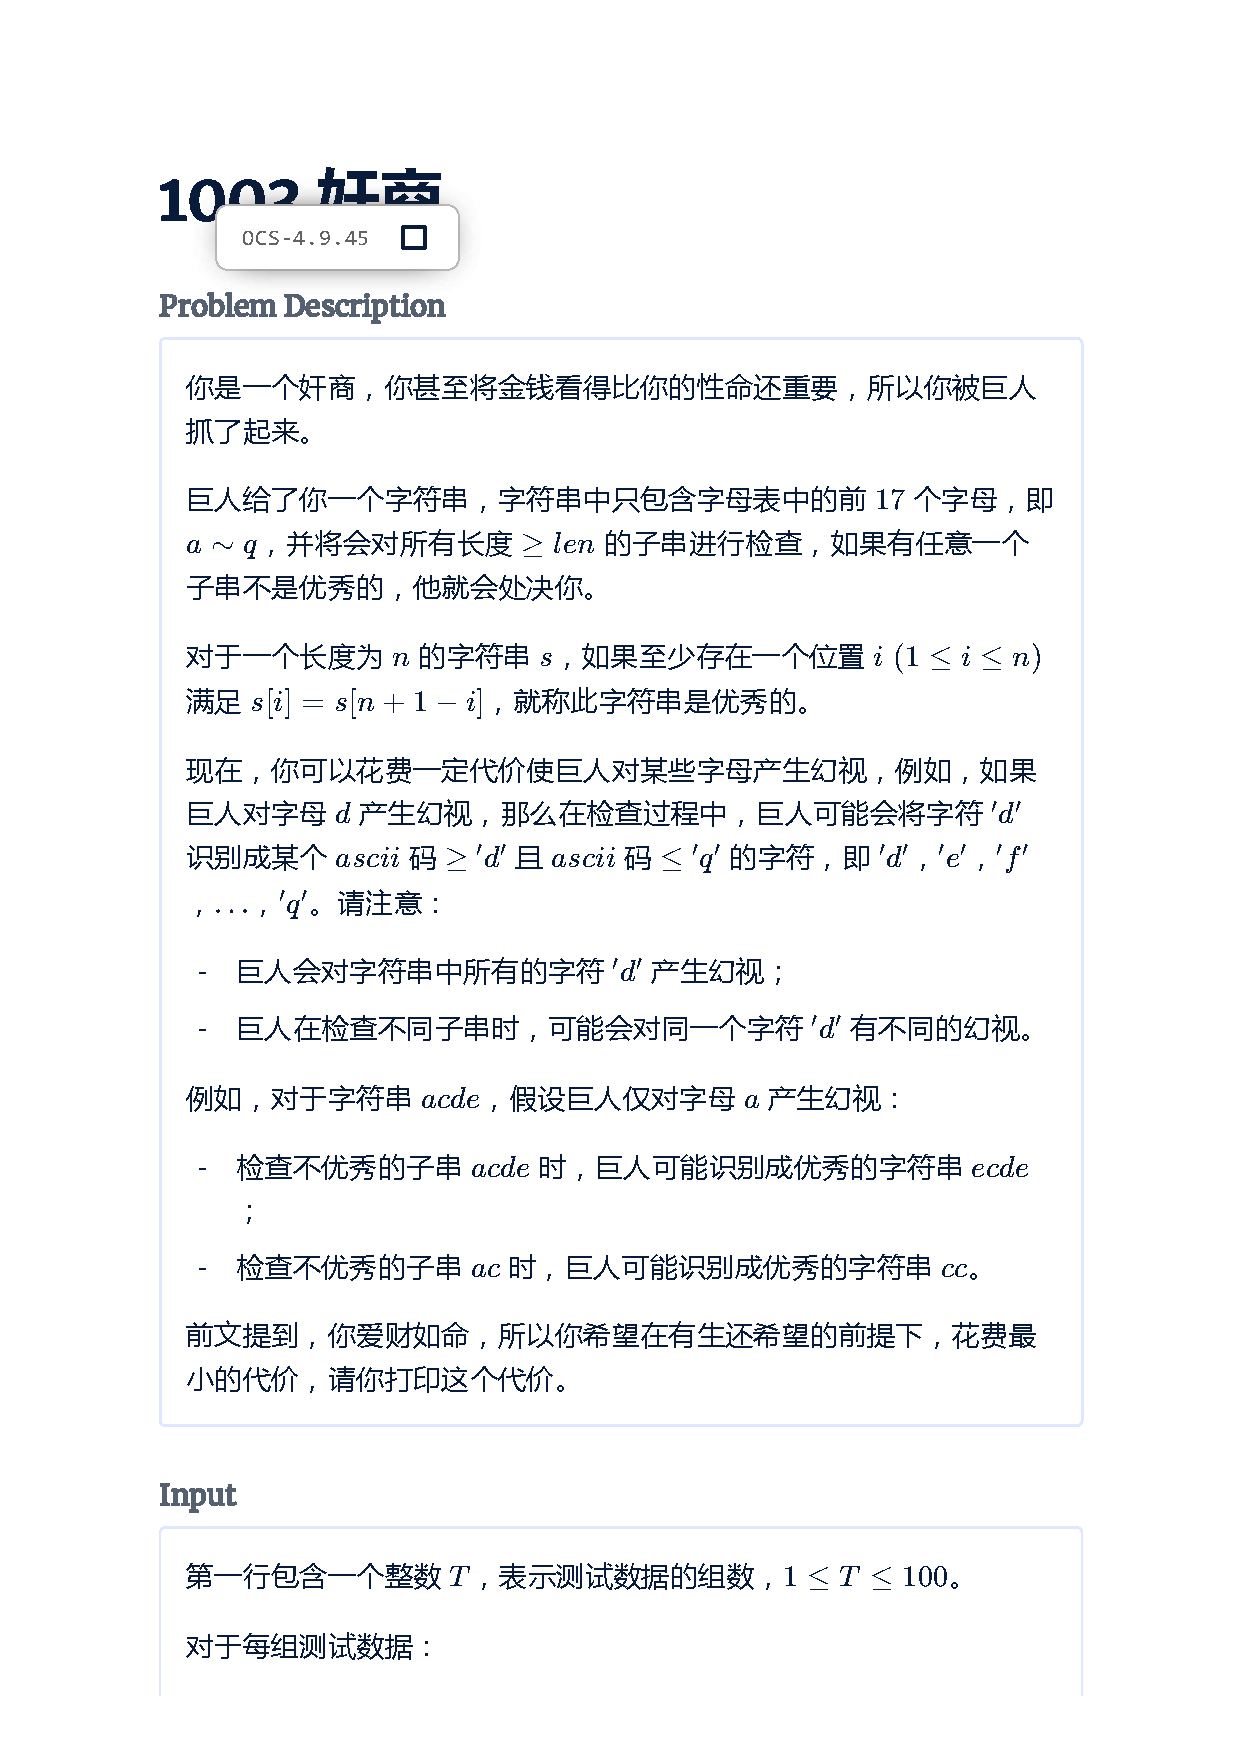
\includegraphics[page=1,width=0.94\linewidth,height=0.90\textheight,keepaspectratio]{assets/pdf/pdf_061.pdf}
\end{center}
\clearpage
\begin{center}
\includegraphics[page=2,width=0.94\linewidth,height=0.90\textheight,keepaspectratio]{assets/pdf/pdf_061.pdf}
\end{center}
\clearpage

\section{区间 DP}
\entrymeta{$O(n^3)$}
\subsection{P4170 {[}CQOI2007{]} 涂色}\label{p4170-cqoi2007-ux6d82ux8272}





\subsection{思路}\label{ux601dux8def}

\[f_{l,r} = min_{i=l}^{r-1}(f_{l,i}+f_{i+1,r})\]


\begin{codeline}
const int N = 55;
int dp[N][N];
char color[N];
int n;
int main() {
    ios::sync_with_stdio(false);
    cin.tie(nullptr);
    cin >> (color);
    memset(dp, 0x3f, sizeof(dp));
    for(; color[n]; n++) {
        dp[n][n] = 1;
    }

    for(int len = 2; len <= n; len++) {
        for(int l = 0; l < n; l++) {
            int r = l + len - 1;

            if(r >= n) {
                break;
            }

            if(color[l] == color[r]) {
                dp[l][r] = min(dp[l + 1][r], dp[l][r - 1]);
            }

            for(int i = l; i < r; i++) {
                dp[l][r] = min(dp[l][r], dp[l][i] + dp[i + 1][r]);
            }
        }
    }

    cout << (dp[0][n - 1]);
}
\end{codeline}


\subsection{P1880 {[}NOI1995{]} 石子合并}\label{p1880-noi1995-ux77f3ux5b50ux5408ux5e76}






\begin{codeline}
#define N 128
int dp[N * 2][N * 2];
int dp2[N * 2][N * 2];
int prefix[N * 2];
int num[N * 2];
int n;

int main() {
    ios::sync_with_stdio(false);
    cin.tie(nullptr);
    cin >> n;
    for(int i = 1; i <= n; i++) {
        cin >> num[i];
        prefix[i] = prefix[i - 1] + num[i];
    }

    for(int i = n + 1; i <= n * 2; i++) {
        num[i] = num[i - n];
        prefix[i] = prefix[i - 1] + num[i];
    }

    for(int l = 2; l <= n; l++) { // [i: i+l]
        for(int i = 1; i <= 2 * n - l + 1; i++) {
            int maximum = 0, minimum = 2147483647;
            for(int j = 1; j < l; j++) {
                maximum = max(maximum, dp[i][i + j - 1] + dp[i + j][i + l - 1]);
                minimum = min(minimum, dp2[i][i + j - 1] + dp2[i + j][i + l - 1]);
            }
            dp[i][i + l - 1] = maximum + prefix[i + l - 1] - prefix[i - 1];
            dp2[i][i + l - 1] = minimum + prefix[i + l - 1] - prefix[i - 1];
        }
    }

    int minimum = 2147483647;
    int maximum = 0;

    for(int i = 1; i <= n; i++) {
        minimum = min(minimum, dp2[i][i + n - 1]);
        maximum = max(maximum, dp[i][i + n - 1]);
    }

    cout << (minimum) << '\n'
         << (maximum) << '\n';
}
\end{codeline}


\subsection{P6934 {[}ICPC 2017 WF{]} Posterize}\label{p6934-icpc-2017-wf-posterize}






\begin{codeline}
const int64 N = 257;
int64 f[N][N];
int64 g[N][N];
int64 pix[N];
int main() {
    ios::sync_with_stdio(false);
    cin.tie(nullptr);
    int64 d, k;
    memset(f, 0x3f, sizeof(f));
    memset(g, 0x3f, sizeof(g));
    cin >> d >> k;
    for(int64 i = 1; i <= d; i++) {
        int64 r, p;
        cin >> r >> p;
        pix[r + 1] = p;
    }

    int64 sum;
    for(int64 i = 1; i < N; i++) {
        for(int64 j = i; j < N; j++) {
            for(int64 t = i; t <= j; t++) {
                sum = 0;
                for(int64 c = i; c <= j; c++) {
                    sum += (c - t) * (c - t) * pix[c];
                }
                f[i][j] = min(f[i][j], sum);
            }
        }
    }

    for(int64 i = 0; i < N; i++) {
        g[i][0] = 0;
    }

    for(int64 i = 1; i <= k; i++) {
        for(int64 r = 1; r < N; r++) {
            for(int64 l = 1; l <= r; l++) {
                g[i][r] = min(g[i][r], g[i - 1][l - 1] + f[l][r]);
            }
        }
    }
    cout << (g[k][N - 1]);
}
\end{codeline}
\begin{warnbox}
按区间长度递增枚举；环形问题拆成 2n。
\end{warnbox}
\clearpage
\subsection*{延伸阅读}
\begin{center}
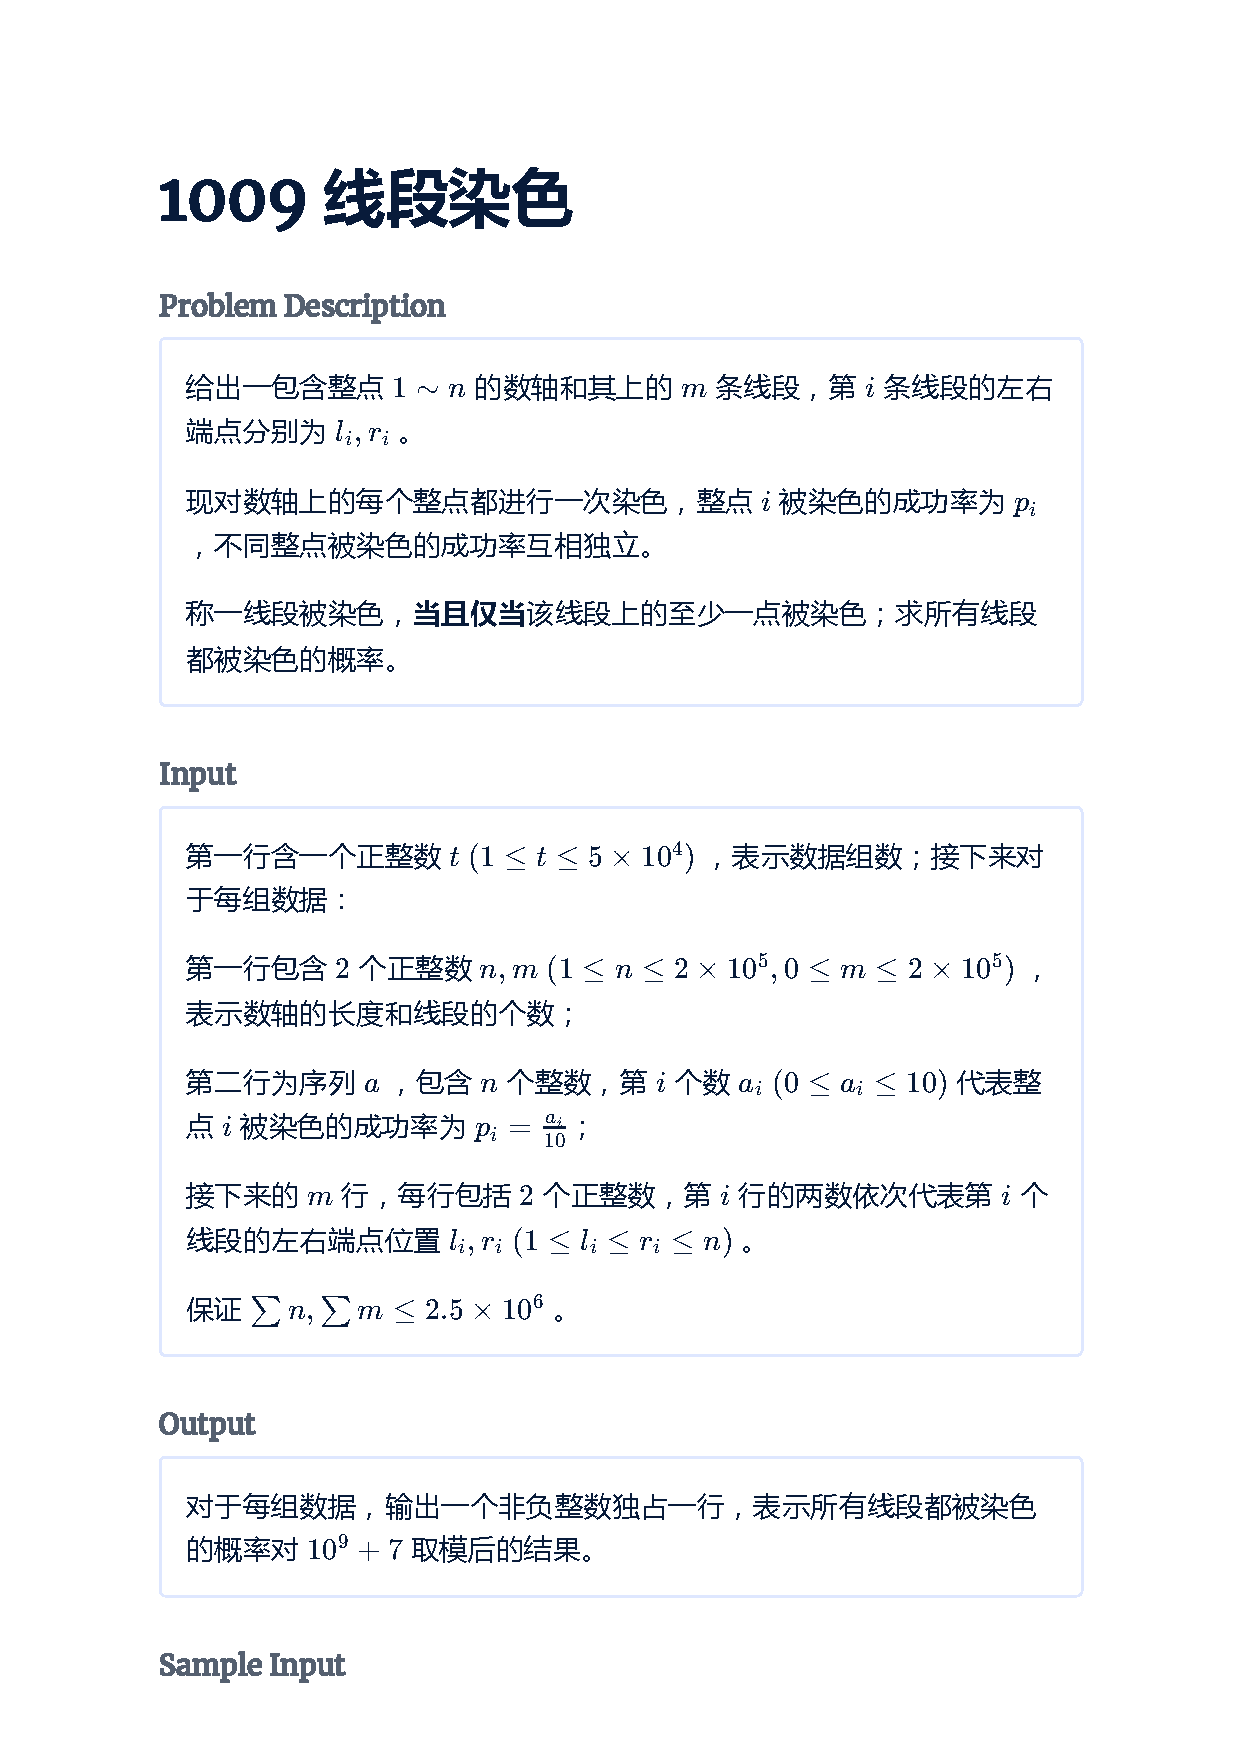
\includegraphics[page=1,width=0.94\linewidth,height=0.90\textheight,keepaspectratio]{assets/pdf/pdf_062.pdf}
\end{center}
\clearpage
\begin{center}
\includegraphics[page=2,width=0.94\linewidth,height=0.90\textheight,keepaspectratio]{assets/pdf/pdf_062.pdf}
\end{center}
\clearpage
\begin{center}
\includegraphics[page=3,width=0.94\linewidth,height=0.90\textheight,keepaspectratio]{assets/pdf/pdf_062.pdf}
\end{center}
\clearpage

\section{树上 DP}
\entrymeta{$O(nm)$}
\subsection{P1642 规划}\label{p1642-ux89c4ux5212}






\begin{codeline}
const int N = 128;
const double ETA = 1e-4;
const double INF = 1e9;

class Node {
public:
    int w, c, s;
    vector<int> oe;
    double dp[N];
};

Node node[N];
int n, m;
double c;

void predfs(int cur, int fa) {
    node[cur].s = 1;
    for(int v : node[cur].oe) {
        if(v != fa) {
            predfs(v, cur);
            node[cur].s += node[v].s;
        }
    }
}

void dfs(int cur, int fa) {
    for(int v : node[cur].oe) {
        if(v != fa) {
            dfs(v, cur);
        }
    }

    node[cur].dp[1] = node[cur].w - node[cur].c * c;
    for(int i = 2; i <= node[cur].s; i++) {
        node[cur].dp[i] = -INF;
    }

    for(int v : node[cur].oe) {
        if(v != fa) {
            for(int i = node[cur].s; i >= 2; i--) {
                for(int j = 1; j <= min(i - 1, node[v].s); j++) {
                    node[cur].dp[i] = max(node[cur].dp[i], node[cur].dp[i - j] + node[v].dp[j]);
                }
            }
        }
    }
\end{codeline}
\vspace{-0.9\baselineskip}
\begin{codeline}[firstnumber=47]
}

bool check() {
    dfs(1, 0);

    for(int i = 1; i <= n; i++) {
        if(node[i].s >= n - m && node[i].dp[n - m] > -ETA) {
            return true;
        }
    }
    return false;
}

int main() {
    ios::sync_with_stdio(false);
    cin.tie(nullptr);
    cin >> n >> m;
    for(int i = 1; i <= n; i++) {
        cin >> node[i].w;
    }

    for(int i = 1; i <= n; i++) {
        cin >> node[i].c;
    }

    int u, v;
    for(int i = 1; i < n; i++) {
        cin >> u >> v;
        node[u].oe.push_back(v);
        node[v].oe.push_back(u);
    }

    predfs(1, 0);

    double ans = 0.;
    double l = 0, r = 10005.0, mid;

    while(abs(r - l) > ETA) {
        c = mid = (l + r) / 2;
        if(check()) {
            ans = l = mid;
        } else {
            r = mid;
        }
    }

\end{codeline}
\vspace{-0.9\baselineskip}
\begin{codeline}[firstnumber=93]
    cout << fixed << setprecision(1) << (ans);
}
\end{codeline}


\subsection{P3478 {[}POI 2008{]} STA-Station}\label{p3478-poi-2008-sta-station}





\paragraph{数据规模与约定}\label{ux6570ux636eux89c4ux6a21ux4e0eux7ea6ux5b9a}

对于全部的测试点，保证 \(1 \leq n \leq 10^6\)，\(1 \leq u, v \leq n\)，给出的是一棵树。


\begin{codeline}
#define N 1000005
int64 n;
class Node {
public:
    vector<int64> son;
    int64 d, w;
    int64 f;
};
Node node[N];

void getWeight(int64 idx, int64 fa) {
    node[idx].w = 1;
    node[idx].f = 0;
    if(fa > 0) {
        node[idx].d = node[fa].d + 1;
    } else {
        node[idx].d = 0;
    }

    for(int64 son : node[idx].son) {
        if(son != fa) {
            getWeight(son, idx);
            node[idx].w += node[son].w;
        }
    }
}

void getSumDep(int64 idx, int64 fa) {
    for(int64 son : node[idx].son) {
        if(son != fa) {
            node[son].f = node[idx].f - node[son].w + (n - node[son].w);
            getSumDep(son, idx);
        }
    }
}

int main() {
    ios::sync_with_stdio(false);
    cin.tie(nullptr);
    cin >> n;
    int64 u, v;
    for(int64 i = 1; i < n; i++) {
        cin >> u >> v;
        node[u].son.push_back(v);
        node[v].son.push_back(u);
    }
\end{codeline}
\vspace{-0.9\baselineskip}
\begin{codeline}[firstnumber=47]

    getWeight(1, -1);

    getSumDep(1, -1);

    int64 ans_idx;
    int64 max_d_sum = -2147483648;

    for(int64 i = 1; i <= n; i++) {
        if(max_d_sum < node[i].f) {
            max_d_sum = node[i].f;
            ans_idx = i;
        }
    }

    cout << (ans_idx) << '\n';
}
\end{codeline}


\subsection{P2014 {[}CTSC1997{]} 选课}\label{p2014-ctsc1997-ux9009ux8bfe}






\begin{codeline}
#define N 305
int n, m;

class Node {
public:
    vector<int> son;
    vector<int> f;
    int score;
};

Node node[305];

int dfs(int root) {
    int s;
    int l = node[root].son.size();
    node[root].f.resize(m + 1, 0);

    if(root == 0) {
        s = 0; // This node itself doesn't count.
        for(int i = 0; i < l; i++) {
            int son = node[root].son[i];
            s += dfs(son);
            for(int j = min(s, m); j >= 0; j--) {
                for(int k = 0; k <= j; k++) {
                    node[root].f[j] = max(node[root].f[j], node[root].f[j - k] + node[son].f[k]);
                }
            }
        }
    } else {
        s = 1; // This node itself.
        node[root].f[1] = node[root].score;
        for(int i = 0; i < l; i++) {
            int son = node[root].son[i];
            s += dfs(son);
            for(int j = min(s, m); j > 0; j--) {
                for(int k = 0; k < j; k++) {
                    node[root].f[j] = max(node[root].f[j], node[root].f[j - k] + node[son].f[k]);
                }
            }
        }
    }
    return s;
}

int main() {
    ios::sync_with_stdio(false);
\end{codeline}
\vspace{-0.9\baselineskip}
\begin{codeline}[firstnumber=47]
    cin.tie(nullptr);
    cin >> n >> m;

    int fa, score;
    for(int i = 1; i <= n; i++) {
        cin >> fa >> score;
        node[fa].son.push_back(i);
        node[i].score = score;
    }

    node[0].score = 0;

    dfs(0);

    cout << (node[0].f[node[0].f.size() - 1]) << '\n';
}
\end{codeline}
\begin{warnbox}
树上背包合并时枚举上界取 \texttt{min(i-1, s[v])}；递归深度可达 1e6。
\end{warnbox}

\section{背包}
\entrymeta{$O(nV)$}
\subsection{引入}\label{ux5f15ux5165}

在具体讲何为「背包 dp」前，先来看如下的例题：

题意概要：有 \(n\) 个物品和一个容量为 \(W\) 的背包，每个物品有重量 \(w_{i}\) 和价值 \(v_{i}\) 两种属性，要求选若干物品放入背包使背包中物品的总价值最大且背包中物品的总重量不超过背包的容量。

在上述例题中，由于每个物体只有两种可能的状态（取与不取），对应二进制中的 \(0\) 和 \(1\)，这类问题便被称为「0-1 背包问题」。

\subsection{0-1 背包}\label{ux80ccux5305}

\subsubsection{解释}\label{ux89e3ux91ca}

例题中已知条件有第 \(i\) 个物品的重量 \(w_{i}\)，价值 \(v_{i}\)，以及背包的总容量 \(W\)。

设 DP 状态 \(f_{i,j}\) 为在只能放前 \(i\) 个物品的情况下，容量为 \(j\) 的背包所能达到的最大总价值。

考虑转移。假设当前已经处理好了前 \(i-1\) 个物品的所有状态，那么对于第 \(i\) 个物品，当其不放入背包时，背包的剩余容量不变，背包中物品的总价值也不变，故这种情况的最大价值为 \(f_{i-1,j}\)；当其放入背包时，背包的剩余容量会减小 \(w_{i}\)，背包中物品的总价值会增大 \(v_{i}\)，故这种情况的最大价值为 \(f_{i-1,j-w_{i}}+v_{i}\)。

由此可以得出状态转移方程：

\[
f_{i,j}=\max(f_{i-1,j},f_{i-1,j-w_{i}}+v_{i})
\]

这里如果直接采用二维数组对状态进行记录，会出现 MLE。可以考虑改用滚动数组的形式来优化。

由于对 \(f_i\) 有影响的只有 \(f_{i-1}\)，可以去掉第一维，直接用 \(f_{i}\) 来表示处理到当前物品时背包容量为 \(i\) 的最大价值，得出以下方程：

\[
f_j=\max \left(f_j,f_{j-w_i}+v_i\right)
\]

\textbf{务必牢记并理解这个转移方程，因为大部分背包问题的转移方程都是在此基础上推导出来的。}

\subsubsection{实现}\label{ux5b9eux73b0}


\begin{codeline}
for(int i = 1; i <= n; i++) {
    for(int l = W; l >= w[i]; l--) {
        f[l] = max(f[l], f[l - w[i]] + v[i]);
    }
}
\end{codeline}


\subsection{完全背包}\label{ux5b8cux5168ux80ccux5305}

\subsubsection{解释}\label{ux89e3ux91ca-1}

完全背包模型与 0-1 背包类似，与 0-1 背包的区别仅在于一个物品可以选取无限次，而非仅能选取一次。

我们可以借鉴 0-1 背包的思路，进行状态定义：设 \(f_{i,j}\) 为只能选前 \(i\) 个物品时，容量为 \(j\) 的背包可以达到的最大价值。

需要注意的是，虽然定义与 0-1 背包类似，但是其状态转移方程与 0-1 背包并不相同。

\subsubsection{过程}\label{ux8fc7ux7a0b}

可以考虑一个朴素的做法：对于第 \(i\) 件物品，枚举其选了多少个来转移。这样做的时间复杂度是 \(O(n^3)\) 的。

状态转移方程如下：

\[
f_{i,j}=\max_{k=0}^{+\infty}(f_{i-1,j-k\times w_i}+v_i\times k)
\]

考虑做一个简单的优化。可以发现，对于 \(f_{i,j}\)，只要通过 \(f_{i,j-w_i}\) 转移就可以了。因此状态转移方程为：

\[
f_{i,j}=\max(f_{i-1,j},f_{i,j-w_i}+v_i)
\]

理由是当我们这样转移时，\(f_{i,j-w_i}\) 已经由 \(f_{i,j-2\times w_i}\) 更新过，那么 \(f_{i,j-w_i}\) 就是充分考虑了第 \(i\) 件物品所选次数后得到的最优结果。换言之，我们通过局部最优子结构的性质重复使用了之前的枚举过程，优化了枚举的复杂度。

与 0-1 背包相同，我们可以将第一维去掉来优化空间复杂度。如果理解了 0-1 背包的优化方式，就不难明白压缩后的循环是正向的（也就是上文中提到的错误优化）。

\subsection{多重背包}\label{ux591aux91cdux80ccux5305}

多重背包也是 0-1 背包的一个变式。与 0-1 背包的区别在于每种物品有 \(k_i\) 个，而非一个。

一个很朴素的想法就是：把「每种物品选 \(k_i\) 次」等价转换为「有 \(k_i\) 个相同的物品，每个物品选一次」。这样就转换成了一个 0-1 背包模型，套用上文所述的方法就可已解决。状态转移方程如下：

\[
f_{i,j}=\max_{k=0}^{k_i}(f_{i-1,j-k\times w_i}+v_i\times k)
\]

时间复杂度 \(O(W\sum_{i=1}^nk_i)\)。


\begin{codeline}
for(int i = 1; i <= n; i++) {
    for(int weight = W; weight >= w[i]; weight--) {
        // 多遍历一层物品数量
        for(int k = 1; k * w[i] <= weight && k <= cnt[i]; k++) {
            dp[weight] = max(dp[weight], dp[weight - k * w[i]] + k * v[i]);
        }
    }
}
\end{codeline}


\subsubsection{二进制分组优化}\label{ux4e8cux8fdbux5236ux5206ux7ec4ux4f18ux5316}

考虑优化。我们仍考虑把多重背包转化成 0-1 背包模型来求解。

\subsubsection{解释}\label{ux89e3ux91ca-2}

显然，复杂度中的 \(O(nW)\) 部分无法再优化了，我们只能从 \(O(\sum k_i)\) 处入手。为了表述方便，我们用 \(A_{i,j}\) 代表第 \(i\) 种物品拆分出的第 \(j\) 个物品。

在朴素的做法中，\(\forall j\le k_i\)，\(A_{i,j}\) 均表示相同物品。那么我们效率低的原因主要在于我们进行了大量重复性的工作。举例来说，我们考虑了「同时选 \(A_{i,1},A_{i,2}\)」与「同时选 \(A_{i,2},A_{i,3}\)」这两个完全等效的情况。这样的重复性工作我们进行了许多次。那么优化拆分方式就成为了解决问题的突破口。

\subsubsection{过程}\label{ux8fc7ux7a0b-1}

我们可以通过「二进制分组」的方式使拆分方式更加优美。

具体地说就是令 \(A_{i,j}\left(j\in\left[0,\lfloor \log_2(k_i+1)\rfloor-1\right]\right)\) 分别表示由 \(2^{j}\) 个单个物品「捆绑」而成的大物品。特殊地，若 \(k_i+1\) 不是 \(2\) 的整数次幂，则需要在最后添加一个由 \(k_i-2^{\lfloor \log_2(k_i+1)\rfloor-1}\) 个单个物品「捆绑」而成的大物品用于补足。

举几个例子：

\begin{itemize}
\tightlist
\item
  \(6=1+2+3\)
\item
  \(8=1+2+4+1\)
\item
  \(18=1+2+4+8+3\)
\item
  \(31=1+2+4+8+16\)
\end{itemize}

显然，通过上述拆分方式，可以表示任意 \(\le k_i\) 个物品的等效选择方式。将每种物品按照上述方式拆分后，使用 0-1 背包的方法解决即可。

时间复杂度 \(O(W\sum_{i=1}^n\log_2k_i)\)

\subsubsection{实现}\label{ux5b9eux73b0-1}


\begin{codeline}
index = 0;
for(int i = 1; i <= m; i++) {
    int c = 1, p, h, k;
    cin >> p >> h >> k;
    while(k > c) {
        k -= c;
        list[++index].w = c * p;
        list[index].v = c * h;
        c *= 2;
    }
    list[++index].w = p * k;
    list[index].v = h * k;
}
\end{codeline}


\subsection{单调队列优化多重背包}\label{ux5355ux8c03ux961fux5217ux4f18ux5316ux591aux91cdux80ccux5305}

???+ note ``问题描述'' 你有 \(n\) 个物品，每个物品重量为 \(w_i\)，价值为 \(v_i\)，数量为 \(k_i\)。你有一个承重上限为 \(W\) 的背包，现在要求你在不超过重量上限的情况下选取价值和尽可能大的物品放入背包。求最大价值。

不了解背包 DP 的请先阅读 \href{../knapsack.md}{背包 DP}。设 \(f_{i,j}\) 表示前 \(i\) 个物品装入承重为 \(j\) 的背包的最大价值，朴素的转移方程为

\[
f_{i,j}=\max_{k=0}^{k_i}(f_{i-1,j-k\times w_i}+v_i\times k)
\]

时间复杂度 \(O(W\sum k_i)\)。

考虑优化 \(f_i\) 的转移。为方便表述，设 \(g_{x,y}=f_{i,x\times w_i+y},g'_{x,y}=f_{i-1,x\times w_i+y}\)，其中 \(0\le y \lt w_i\)，则转移方程可以表示为：

\[
g_{x,y}=\max_{k=0}^{k_i}(g'_{x-k,y}+v_i\times k)
\]

设 \(G_{x,y}=g'_{x,y}-v_i\times x\)。则方程可以表示为：

\[
g_{x,y}=\max_{k=0}^{k_i}(G_{x-k,y})+v_i\times x
\]

这样就转化为一个经典的单调队列优化形式了。\(G_{x,y}\) 可以 \(O(1)\) 计算，因此对于固定的 \(y\)，我们可以在 \(O\left( \left\lfloor \dfrac{W}{w_i} \right\rfloor \right)\) 的时间内计算出 \(g_{x,y}\)。因此求出所有 \(g_{x,y}\) 的复杂度为 \(O\left( \left\lfloor \dfrac{W}{w_i} \right\rfloor \right)\times O(w_i)=O(W)\)。这样转移的总复杂度就降为 \(O(nW)\)。

在实现的时候，我们需要先枚举 \(y\)，这样才能保证枚举 \(x\) 的时候利用单调队列进行优化，而单调队列中存储的是 \(x-k\)，并不存储 \(k\)，这样使用的时候需要通过 \texttt{f{[}last{]}{[}q.front()\ *\ w{[}i{]}\ +\ y{]}\ -\ q.front()\ *\ v{[}i{]}} 获取对应的 \(G_{x-k,y}\)，不难发现 \(x-k\in [x - k_i,x]\)，因此在枚举 \(x\) 的时候，我们需要删除队列中不在这个范围内的元素。


\begin{codeline}
constexpr int MAXV = 4e4 + 10;
constexpr int MAXN = 1e2 + 10;
int n, W, last = 0, now = 1;
int v[MAXN], w[MAXN], k[MAXN];
int f[2][MAXV];
deque<int> q;

int main() {
    ios::sync_with_stdio(false);
    cin >> n >> W;
    for(int i = 1; i <= n; i++) {
        cin >> v[i] >> w[i] >> k[i];
    }
    for(int i = 1; i <= n; i++) {
        for(int y = 0; y < w[i]; y++) {
            // 清空队列
            deque<int>().swap(q);
            for(int x = 0; x * w[i] + y <= W; x++) {
                // 弹出不在范围的元素
                while(!q.empty() && q.front() < x - k[i]) {
                    q.pop_front();
                }
                // 保证队列单调
                while(!q.empty() && f[last][q.back() * w[i] + y] - q.back() * v[i] <
                                        f[last][x * w[i] + y] - x * v[i]) {
                    q.pop_back();
                }
                q.push_back(x);
                f[now][x * w[i] + y] =
                    f[last][q.front() * w[i] + y] - q.front() * v[i] + x * v[i];
            }
        }
        swap(last, now);
    }
    cout << f[last][W] << endl;
    return 0;
}
\end{codeline}


\subsection{混合背包}\label{ux6df7ux5408ux80ccux5305}

混合背包就是将前面三种的背包问题混合起来，有的只能取一次，有的能取无限次，有的只能取 \(k\) 次。

这种题目看起来很吓人，可是只要领悟了前面几种背包的中心思想，并将其合并在一起就可以了。下面给出伪代码：



\subsection{二维费用背包}\label{ux4e8cux7ef4ux8d39ux7528ux80ccux5305}

有 \(n\) 个任务需要完成，完成第 \(i\) 个任务需要花费 \(t_i\) 分钟，产生 \(c_i\) 元的开支。

现在有 \(T\) 分钟时间，\(W\) 元钱来处理这些任务，求最多能完成多少任务。

这道题是很明显的 0-1 背包问题，可是不同的是选一个物品会消耗两种价值（经费、时间），只需在状态中增加一维存放第二种价值即可。

这时候就要注意，再开一维存放物品编号就不合适了，因为容易 MLE。

\subsubsection{实现}\label{ux5b9eux73b0-2}


\begin{codeline}
for(int k = 1; k <= n; k++) {
    for(int i = m; i >= mi; i--) {     // 对经费进行一层枚举
        for(int j = t; j >= ti; j--) { // 对时间进行一层枚举
            dp[i][j] = max(dp[i][j], dp[i - mi][j - ti] + 1);
        }
    }
}
\end{codeline}


\subsection{分组背包}\label{ux5206ux7ec4ux80ccux5305}

有 \(n\) 件物品和一个大小为 \(m\) 的背包，第 \(i\) 个物品的价值为 \(w_i\)，体积为 \(v_i\)。同时，每个物品属于一个组，同组内最多只能选择一个物品。求背包能装载物品的最大总价值。

这种题怎么想呢？其实是从「在所有物品中选择一件」变成了「从当前组中选择一件」，于是就对每一组进行一次 0-1 背包就可以了。

再说一说如何进行存储。我们可以将 \(t_{k,i}\) 表示第 \(k\) 组的第 \(i\) 件物品的编号是多少，再用 \(\mathit{cnt}_k\) 表示第 \(k\) 组物品有多少个。

\subsubsection{实现}\label{ux5b9eux73b0-3}


\begin{codeline}
for(int k = 1; k <= ts; k++) {             // 循环每一组
    for(int i = m; i >= 0; i--) {          // 循环背包容量
        for(int j = 1; j <= cnt[k]; j++) { // 循环该组的每一个物品
            if(i >= w[t[k][j]]) {          // 背包容量充足
                dp[i] = max(dp[i],
                            dp[i - w[t[k][j]]] + c[t[k][j]]); // 像0-1背包一样状态转移
            }
        }
    }
}
\end{codeline}


这里要注意：\textbf{一定不能搞错循环顺序}，这样才能保证正确性。

\subsection{有依赖的背包}\label{ux6709ux4f9dux8d56ux7684ux80ccux5305}

金明有 \(n\) 元钱，想要买 \(m\) 个物品，第 \(i\) 件物品的价格为 \(v_i\)，重要度为 \(p_i\)。有些物品是从属于某个主件物品的附件，要买这个物品，必须购买它的主件。

目标是让所有购买的物品的 \(v_i \times p_i\) 之和最大。

考虑分类讨论。对于一个主件和它的若干附件，有以下几种可能：只买主件，买主件 + 某些附件。因为这几种可能性只能选一种，所以可以将这看成分组背包。

如果是多叉树的集合，则要先算子节点的集合，最后算父节点的集合。

\subsection{泛化物品的背包}\label{ux6cdbux5316ux7269ux54c1ux7684ux80ccux5305}

这种背包，没有固定的费用和价值，它的价值是随着分配给它的费用而定。在背包容量为 \(V\) 的背包问题中，当分配给它的费用为 \(v_i\) 时，能得到的价值就是 \(h\left(v_i\right)\)。这时，将固定的价值换成函数的引用即可。

\subsection{杂项}\label{ux6742ux9879}

\subsubsection{小优化}\label{ux5c0fux4f18ux5316}

根据贪心原理，当费用相同时，只需保留价值最高的；当价值一定时，只需保留费用最低的；当有两件物品 \(i,j\) 且 \(i\) 的价值大于 \(j\) 的价值并且 \(i\) 的费用小于 \(j\) 的费用时，只需保留 \(i\)。

\subsubsection{背包问题变种}\label{ux80ccux5305ux95eeux9898ux53d8ux79cd}

\paragraph{输出方案}\label{ux8f93ux51faux65b9ux6848}

输出方案其实就是记录下来背包中的某一个状态是怎么推出来的。我们可以用 \(g_{i,v}\) 表示第 \(i\) 件物品占用空间为 \(v\) 的时候是否选择了此物品。然后在转移时记录是选用了哪一种策略（选或不选）。输出时的伪代码：


\begin{codeline}
int v = V; // 记录当前的存储空间

// 因为最后一件物品存储的是最终状态，所以从最后一件物品进行循环
for(从最后一件循环至第一件) {
    if(g[i][v]) {
        选了第 i 项物品;
        v -= 第 i 项物品的重量;
    } else {
        未选第 i 项物品;
    }
}
\end{codeline}


\paragraph{求方案数}\label{ux6c42ux65b9ux6848ux6570}

对于给定的一个背包容量、物品费用、其他关系等的问题，求装到一定容量的方案总数。

这种问题就是把求最大值换成求和即可。

例如 0-1 背包问题的转移方程就变成了：

\[
\mathit{dp}_i=\sum(\mathit{dp}_i,\mathit{dp}_{i-c_i})
\]

初始条件：\(\mathit{dp}_0=1\)

因为当容量为 \(0\) 时也有一个方案，即什么都不装。

\paragraph{求最优方案总数}\label{ux6c42ux6700ux4f18ux65b9ux6848ux603bux6570}

要求最优方案总数，我们要对 0-1 背包里的 \(\mathit{dp}\) 数组的定义稍作修改，DP 状态 \(f_{i,j}\) 为在只能放前 \(i\) 个物品的情况下，容量为 \(j\) 的背包「正好装满」所能达到的最大总价值。

这样修改之后，每一种 DP 状态都可以用一个 \(g_{i,j}\) 来表示方案数。

\(f_{i,j}\) 表示只考虑前 \(i\) 个物品时背包体积「正好」是 \(j\) 时的最大价值。

\(g_{i,j}\) 表示只考虑前 \(i\) 个物品时背包体积「正好」是 \(j\) 时的方案数。

转移方程：

如果 \(f_{i,j} = f_{i-1,j}\) 且 \(f_{i,j} \neq f_{i-1,j-v}+w\) 说明我们此时不选择把物品放入背包更优，方案数由 \(g_{i-1,j}\) 转移过来，

如果 \(f_{i,j} \neq f_{i-1,j}\) 且 \(f_{i,j} = f_{i-1,j-v}+w\) 说明我们此时选择把物品放入背包更优，方案数由 \(g_{i-1,j-v}\) 转移过来，

如果 \(f_{i,j} = f_{i-1,j}\) 且 \(f_{i,j} = f_{i-1,j-v}+w\) 说明放入或不放入都能取得最优解，方案数由 \(g_{i-1,j}\) 和 \(g_{i-1,j-v}\) 转移过来。

初始条件：


\begin{codeline}
memset(f, -0x3f, sizeof(f)); // 最大值 DP 的不可达哨兵，避免未装满状态参与转移
f[0] = 0;
g[0] = 1; // 什么都不装是一种方案
\end{codeline}


因为背包体积最大值有可能装不满，所以最优解不一定是 \(f_{m}\)。

最后我们通过找到最优解的价值，把 \(g_{j}\) 数组里取到最优解的所有方案数相加即可。


\begin{codeline}
for(int i = 0; i < N; i++) {
    for(int j = V; j >= v[i]; j--) {
        int tmp = max(dp[j], dp[j - v[i]] + w[i]);
        int c = 0;
        if(tmp == dp[j]) {
            c += cnt[j]; // 如果从dp[j]转移
        }
        if(tmp == dp[j - v[i]] + w[i]) {
            c += cnt[j - v[i]]; // 如果从dp[j-v[i]]转移
        }
        dp[j] = tmp;
        cnt[j] = c;
    }
}
int ans = 0; // 寻找最优解
for(int i = 0; i <= V; i++) {
    ans = max(ans, dp[i]);
}
int res = 0;
for(int i = 0; i <= V; i++) {
    if(dp[i] == ans) {
        res += cnt[i]; // 求和最优解方案数
    }
}
\end{codeline}


\paragraph{背包的第 k 优解}\label{ux80ccux5305ux7684ux7b2c-k-ux4f18ux89e3}

普通的 0-1 背包是要求最优解，在普通的背包 DP 方法上稍作改动，增加一维用于记录当前状态下的前 k 优解，即可得到求 0-1 背包第 \(k\) 优解的算法。 具体来讲：\(\mathit{dp_{i,j,k}}\) 记录了前 \(i\) 个物品中，选择的物品总体积为 \(j\) 时，能够得到的第 \(k\) 大的价值和。这个状态可以理解为将普通 0-1 背包只用记录一个数据的 \(\mathit{dp_{i,j}}\) 扩展为记录一个有序的优解序列。转移时，普通背包最优解的求法是 \(\mathit{dp_{i,j}}=\max(\mathit{dp_{i-1,j}},\mathit{dp_{i-1,j-v_{i}}}+w_{i})\)，现在我们则是要合并 \(\mathit{dp_{i-1,j}}\)，\(\mathit{dp_{i-1,j-v_{i}}}+w_{i}\) 这两个大小为 \(k\) 的递减序列，并保留合并后前 \(k\) 大的价值记在 \(\mathit{dp_{i,j}}\) 里，这一步利用双指针法，复杂度是 \(O(k)\) 的，整体时间复杂度为 \(O(nmk)\)。空间上，此方法与普通背包一样可以压缩掉第一维，复杂度是 \(O(mk)\) 的。


\begin{codeline}
memset(dp, 0, sizeof(dp));
int i, j, p, x, y, z;
cin >> n >> m >> K;
for(i = 0; i < n; i++) {
    cin >> w[i];
}
for(i = 0; i < n; i++) {
    cin >> c[i];
}
for(i = 0; i < n; i++) {
    for(j = m; j >= c[i]; j--) {
        for(p = 1; p <= K; p++) {
            a[p] = dp[j - c[i]][p] + w[i];
            b[p] = dp[j][p];
        }
        a[p] = b[p] = -1;
        x = y = z = 1;
        while(z <= K && (a[x] != -1 || b[y] != -1)) {
            if(a[x] > b[y]) {
                dp[j][z] = a[x++];
            } else {
                dp[j][z] = b[y++];
            }
            if(dp[j][z] != dp[j][z - 1]) {
                z++;
            }
        }
    }
}
cout << (dp[m][K]) << '\n';
\end{codeline}


\subsection{P1417 烹调方案}\label{p1417-ux70f9ux8c03ux65b9ux6848}






\begin{codeline}
#define N 64
int64 t, n;

class Item {
public:
    int64 a, b, c;
};

bool operator<(const Item& A, const Item& B) {
    return A.c * B.b < A.b * B.c;
}

Item item[N];

int64 dp[100005];

int main() {
    ios::sync_with_stdio(false);
    cin.tie(nullptr);
    cin >> t >> n;
    for(int64 i = 0; i < n; i++) {
        cin >> item[i].a;
    }

    for(int64 i = 0; i < n; i++) {
        cin >> item[i].b;
    }

    for(int64 i = 0; i < n; i++) {
        cin >> item[i].c;
    }

    sort(item, item + n);

    for(int64 i = 0; i < n; i++) {
        for(int64 j = t; j >= 0; j--) {
            if(j - item[i].c >= 0) {
                dp[j] = max(dp[j - item[i].c] + item[i].a - item[i].b * j, dp[j]);
            }
        }
    }

    int64 maximum = 0;

    for(int64 i = 0; i <= t; i++) {
        maximum = max(maximum, dp[i]);
\end{codeline}
\vspace{-0.9\baselineskip}
\begin{codeline}[firstnumber=47]
    }
    cout << (maximum);
}
\end{codeline}
\begin{warnbox}
0/1 背包容量倒序；「恰好装满」的最大值 DP 用负哨兵（\texttt{memset(f, -0x3f, ...)}），不要用正无穷。
\end{warnbox}

\section{SOSDP}
\entrymeta{$O(n\cdot 2^{\omega(x)})$}
\begin{center}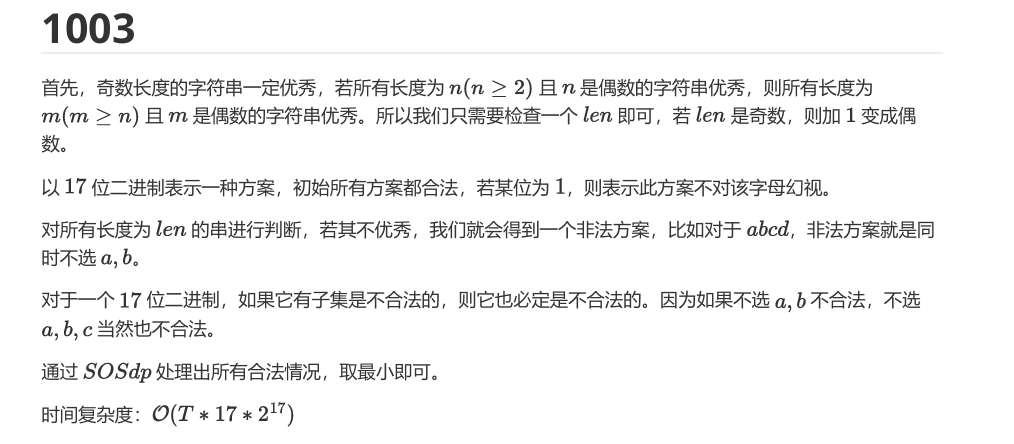
\includegraphics[width=0.78\linewidth]{assets/e065_image.png}\end{center}


\begin{codeline}
const int N = 100005;
int n, x;

inline int gcd(int a, int b) {
    if(b == 0) {
        return a;
    } else {
        return gcd(b, a % b);
    }
}

inline long long lcm(int a, int b) {
    return 1LL * a / gcd(a, b) * b;
}

class Node {
public:
    vector<int> oe;
    int b;
    int f[1 << 8];
};

Node node[N];

int p[8];
int k[8];
int pcnt;
long long ans;

void dfs(int cur, int fa) {
    if(node[cur].b != -1) {
        node[cur].f[node[cur].b] = 1;
        if(node[cur].b == (1 << pcnt) - 1) {
            ans++;
        }

        for(int v : node[cur].oe) {
            if(v != fa) {
                int s[1 << pcnt];
                for(int i = 0; i < 1 << pcnt; i++) {
                    s[i] = node[cur].f[i];
                }

                for(int j = 0; j < pcnt; j++) {
                    for(int i = 0; i < 1 << pcnt; i++) {
                        if(!(i & (1 << j))) {
\end{codeline}
\vspace{-0.9\baselineskip}
\begin{codeline}[firstnumber=47]
                            s[i] += s[i ^ (1 << j)];
                        }
                    }
                }

                dfs(v, cur);
                if(node[v].b != -1) {
                    for(int i = 0; i < 1 << pcnt; i++) {
                        ans += 1ll * s[((1 << pcnt) - 1) ^ (i | node[cur].b)] * node[v].f[i];
                        node[cur].f[i | node[cur].b] += node[v].f[i];
                    }
                }
            }
        }
    } else {
        for(int v : node[cur].oe) {
            if(v != fa) {
                dfs(v, cur);
            }
        }
    }
}

int main() {
    ios::sync_with_stdio(false);
    cin.tie(nullptr);
    int T;
    cin >> T;
    while(T--) {
        cin >> n >> x;
        pcnt = 0;
        ans = 0;
        for(int i = 0; i < 8; i++) {
            k[i] = p[i] = 0;
        }
        int a = x;
        for(int i = 2; 1LL * i * i <= a; i++) {
            if(a % i == 0) {
                p[pcnt] = i;
                while(a % i == 0) {
                    a /= i;
                    k[pcnt]++;
                }
                pcnt++;
            }
        }
\end{codeline}
\vspace{-0.9\baselineskip}
\begin{codeline}[firstnumber=93]
        if(a > 1) {
            p[pcnt] = a;
            k[pcnt] = 1;
            pcnt++;
        }

        for(int i = 1; i <= n; i++) {
            node[i].oe.clear();
            node[i].b = 0;
            for(int j = 0; j < 1 << pcnt; j++) {
                node[i].f[j] = 0;
            }
        }

        int u, v;
        for(int i = 1; i < n; i++) {
            cin >> u >> v;
            node[u].oe.push_back(v);
            node[v].oe.push_back(u);
        }

        for(int i = 1; i <= n; i++) {
            cin >> a;
            if(lcm(a, x) != x) {
                node[i].b = -1;
            } else {
                for(int j = 0; j < pcnt; j++) {
                    int cnt = 0;
                    while(a % p[j] == 0) {
                        a /= p[j];
                        cnt++;
                    }
                    if(cnt == k[j]) {
                        node[i].b |= 1 << j;
                    }
                }
            }
        }

        dfs(1, 0);
        cout << (ans) << '\n';
    }
}
\end{codeline}


\begin{center}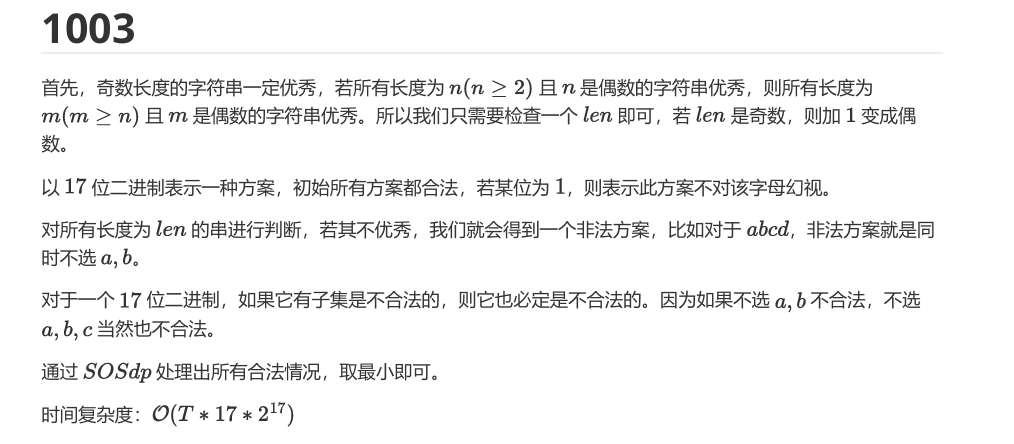
\includegraphics[width=0.78\linewidth]{assets/e065_image.png}\end{center}


\begin{codeline}
const int N = 3005;
const int K = 17;
int n;
int l;

char s[N];
int w[K];
bool legal[1 << K];
int cost(int state) {
    int tot = 0;
    for(int i = 0; i < K; i++) {
        if(!(state & (1 << i))) {
            tot += w[i];
        }
    }
    return tot;
}

int main() {
    ios::sync_with_stdio(false);
    cin.tie(nullptr);
    int T;
    cin >> T;
    while(T--) {
        cin >> n;
        cin >> (s);
        for(int i = 0; i < K; i++) {
            cin >> w[i];
        }
        cin >> l;

        if(l & 1) {
            l++;
        }

        if(l > n) {
            cout << (0) << '\n';
        } else {
            memset(legal, 1, sizeof(legal));
            for(int i = 0; i + l <= n; i++) {
                int state = 0;
                for(int j = 0; j < l / 2; j++) {
                    if(s[i + j] == s[i + l - 1 - j]) {
                        state = 0;
                        break;
                    } else {
\end{codeline}
\vspace{-0.9\baselineskip}
\begin{codeline}[firstnumber=47]
                        char mini = min(s[i + j], s[i + l - 1 - j]);
                        state |= 1 << (mini - 'a');
                    }
                }
                if(state) {
                    legal[state] = false;
                }
            }

            for(int j = 0; j < K; j++) {
                for(int i = 0; i < 1 << K; i++) {
                    if(i & (1 << j)) {
                        legal[i] &= legal[i ^ (1 << j)];
                    }
                }
            }

            int ans = 0x3f3f3f3f;
            for(int i = 0; i < 1 << K; i++) {
                if(legal[i]) {
                    ans = min(ans, cost(i));
                }
            }

            cout << (ans) << '\n';
        }
    }
}
\end{codeline}
\begin{warnbox}
x ≤ 1e7 最多 8 个不同质因子；\texttt{lcm} 用 \texttt{1LL * a / gcd * b}，分解到 \texttt{i*i \textless{}= a}。
\end{warnbox}
\clearpage
\subsection*{延伸阅读}
\begin{center}
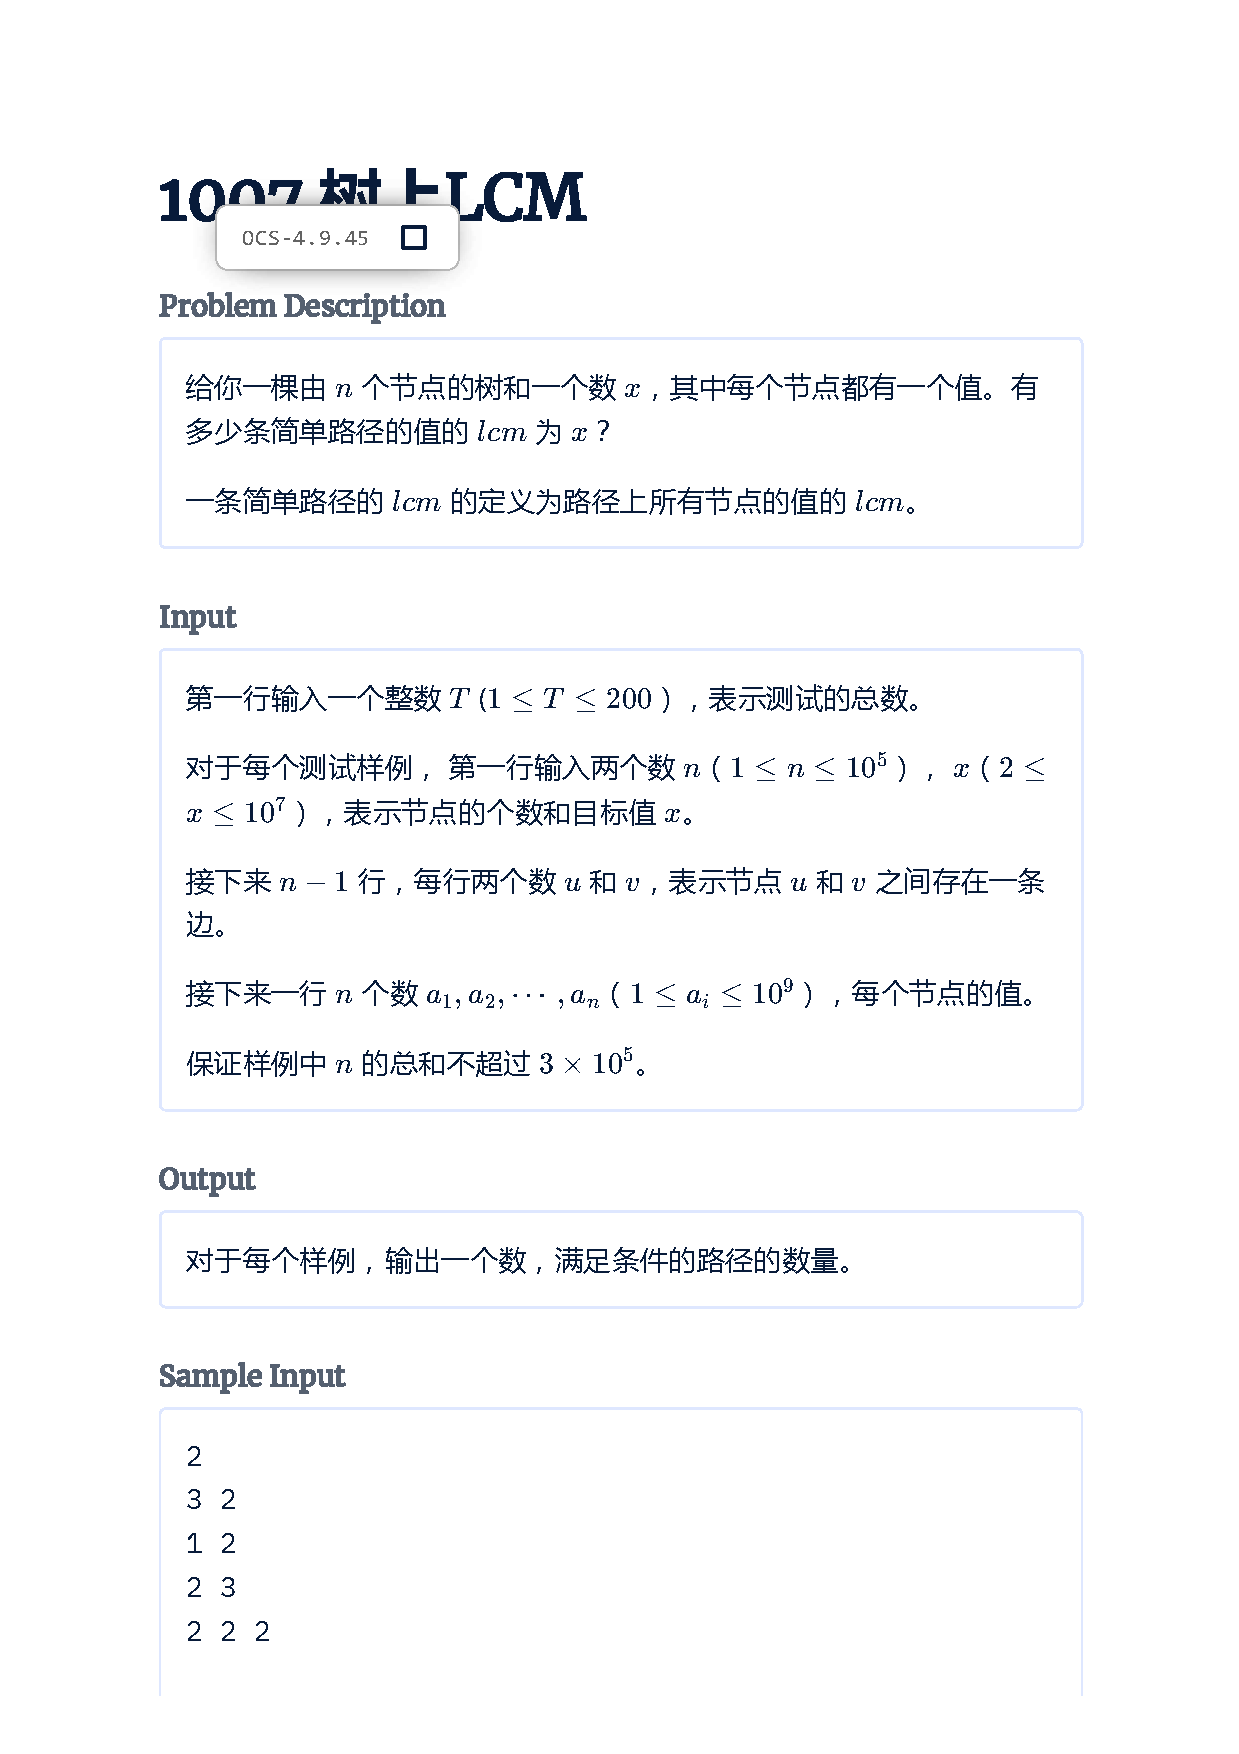
\includegraphics[page=1,width=0.94\linewidth,height=0.90\textheight,keepaspectratio]{assets/pdf/pdf_065.pdf}
\end{center}
\clearpage
\begin{center}
\includegraphics[page=2,width=0.94\linewidth,height=0.90\textheight,keepaspectratio]{assets/pdf/pdf_065.pdf}
\end{center}
\clearpage

\section{DP 优化}
\entrymeta{$O(n\log n)$ / $O(nm)$}
\subsection{P3216 {[}HNOI2011{]} 数学作业}\label{p3216-hnoi2011-ux6570ux5b66ux4f5cux4e1a}






\begin{codeline}
const uint64 N = 3;
uint64 n, m;

class Matrix {
public:
    uint64 arr[N][N];

    Matrix operator*(const Matrix& o) {
        Matrix res = {0};

        for(uint64 i = 0; i < N; i++) {
            for(uint64 j = 0; j < N; j++) {
                for(uint64 k = 0; k < N; k++) {
                    res.arr[i][j] += arr[i][k] * o.arr[k][j];
                }
                res.arr[i][j] %= m;
            }
        }

        return res;
    }
};
Matrix A, B;
Matrix E = {
    1, 0, 0,
    0, 1, 0,
    0, 0, 1};

int main() {
    ios::sync_with_stdio(false);
    cin.tie(nullptr);
    cin >> n >> m;

    A.arr[0][0] = 0;
    A.arr[1][0] = 1;
    A.arr[2][0] = 1;
    B.arr[0][1] = 1;
    B.arr[1][1] = 1;
    B.arr[1][2] = 1;
    B.arr[2][2] = 1;

    for(uint64 i = 1; i <= n; i *= 10) {
        B.arr[0][0] = i * 10 % m;
        A = quickPow(B, min(n + 1, i * 10) - i, E) * A;
    }

\end{codeline}
\vspace{-0.9\baselineskip}
\begin{codeline}[firstnumber=47]
    cout << (A.arr[0][0]) << '\n';
}
\end{codeline}


\subsection{P2513 {[}HAOI2009{]} 逆序对数列}\label{p2513-haoi2009-ux9006ux5e8fux5bf9ux6570ux5217}






\begin{codeline}
const int MODER = 10000;
const int N = 1024;
int dp[N][N];

int main() {
    ios::sync_with_stdio(false);
    cin.tie(nullptr);
    int n, k;
    cin >> n >> k;

    dp[0][0] = 1;
    for(int i = 0; i < n; i++) {

        for(int j = 1; j <= k; j++) {
            dp[i][j] += dp[i][j - 1];
            dp[i][j] %= MODER;
        }

        for(int j = 0; j <= k; j++) {
            int l = j - min(i, j) - 1;
            if(l < 0) {
                dp[i + 1][j] = dp[i][j];
            } else {
                dp[i + 1][j] = (dp[i][j] - dp[i][l] + MODER) % MODER;
            }
        }
    }
    cout << (dp[n][k] % MODER) << '\n';
}
\end{codeline}
\begin{warnbox}
矩阵快速幂按位数分组；斜率优化注意单调性前提。
\end{warnbox}

